\documentclass[uplatex,dvipdfmx]{jsarticle}
\usepackage[top=20truemm,bottom=20truemm,left=25truemm,right=25truemm]{geometry}
\usepackage{graphicx}

\usepackage[noto]{pxchfon}	%for use Noto fonts
\usepackage{multirow}
\usepackage{here}
\usepackage{threeparttable}
\usepackage{array}

\title{KOSENation CUP VALORANT プレイヤーブック}
\author{\hfill 3rdJCG, ayana``}
\date{\today}

\begin{document}

\maketitle

\section{まえがき}
	本大会での試合形式や注意点についてまとめました。
	試合の間などの短い時間でも確認できるようダウンロードや印刷などを行うことを推奨します。

\section{グループマッチ}
	1日目はグループAとBの2つのグループに分かれ、そのグループ内で総当たりの試合を行います。当日はすべてのチームが5つの試合を行う予定です。

	\begin{table}[htbp]
	    \centering
	    \caption{グループ表}
	    \begin{tabular}{p{10zw}|p{10zw}}
	        \hline
	        {\bf グループA}       & {\bf グループB}  \\ \hline
	        死後、お見知り置きを  & 黄金比果実       \\ \hline
	        三寒四温              & Wither           \\ \hline
	        The KOSENATOR         & Team Hell-SEA    \\ \hline
	        Noah                  & storm            \\ \hline
	        5Ms                   & 未定             \\ \hline
	        Funny Creators        & キャ虐は人生     \\ \hline
	    \end{tabular}
	\end{table}


	\subsection{対戦表}
	    対戦表を以下に示します。すべてのチームがすべての時間帯で試合がありますので、注意してください。

	    \newpage
	    \begin{center}
	        \begin{threeparttable}[h]
	            \begin{table}[H]
	                \caption{グループAの対戦表}
	                \begin{tabular}{p{4zw}|p{5zw}|Wc{3zw}|p{10zw}|p{10zw}}
	                    \hline
	                    {\bf 時刻} \tnote{*}      & {\bf 試合番号}            & \multicolumn{1}{l|}{{\bf Ch.}}  & {\bf Team 1}    & {\bf Team 2}          \\ \hline
	                    \multirow{3}{*}{10:00 -}  & GA-1A                     & A                               & 三寒四温        & 死後、お見知りおきを  \\ \cline{2-5}
	                                              & GA-1B                     & B                               & Noah            & The KOSENATOR         \\ \cline{2-5}
	                                              & GA-1C                     & C                               & Funny Creators  & 5Ms                   \\ \hline
	                    \multirow{3}{*}{11:20 -}  & GA-2A                     & A                               & The KOSENATOR   & 死後、お見知り置きを  \\ \cline{2-5}
	                                              & GA-2B                     & B                               & 5Ms             & 三寒四温              \\ \cline{2-5}
	                                              & GA-2C                     & C                               & Funny Creators  & Noah                  \\ \hline
	                                              & \multicolumn{4}{c}{休憩}                                                                              \\ \hline
	                    \multirow{3}{*}{13:20 -}  & GA-3A \tnote{\bf 配信}    & A                               & Noah            & 三寒四温              \\ \cline{2-5}
	                                              & GA-3B                     & B                               & 5Ms             & 死後、お見知り置きを  \\ \cline{2-5}
	                                              & GA-3C                     & C                               & Funny Creators  & The KOSENATOR         \\ \hline
	                    \multirow{3}{*}{14:40 -}  & GA-4A                     & A                               & Noah            & 死後、お見知り置きを  \\ \cline{2-5}
	                                              & GA-4B \tnote{\bf 配信}    & B                               & 5Ms             & The KOSENATOR         \\ \cline{2-5}
	                                              & GA-4C                     & C                               & Funny Creators  & 三寒四温              \\ \hline
	                    \multirow{3}{*}{16:00 -}  & GA-5A                     & A                               & The KOSENATOR   & 三寒四温              \\ \cline{2-5}
	                                              & GA-5B                     & B                               & 5Ms             & Noah                  \\ \cline{2-5}
	                                              & GA-5C \tnote{\bf 配信}    & C                               & Funny Creators  & 死後、お見知り置きを  \\ \hline
	                \end{tabular}
	            \end{table}
	            \begin{tablenotes}
	                \item[*] 時刻は試合状況に応じて変更される可能性があります
	                \item[配信] 配信試合です
	            \end{tablenotes}
	        \end{threeparttable}
	    \end{center}

	    \begin{center}
	        \begin{threeparttable}[h]
	            \begin{table}[H]
	                \caption{グループBの対戦表}
	                \begin{tabular}{p{4zw}|p{5zw}|Wc{3zw}|p{10zw}|p{10zw}}
	                    \hline
	                    {\bf 時刻} \tnote{*}      & {\bf 試合番号}            & \multicolumn{1}{l|}{{\bf Ch.}}  & {\bf Team 1}   & {\bf Team 2}   \\ \hline
	                    \multirow{3}{*}{10:00 -}  & GB-1D \tnote{\bf 配信}    & D                               & Wither         & 黄金比果実     \\ \cline{2-5}
	                                              & GB-1E                     & E                               & storm          & Team Hell-SEA  \\ \cline{2-5}
	                                              & GB-1F                     & F                               & キャ虐は人生   & 未定           \\ \hline
	                    \multirow{3}{*}{11:20 -}  & GB-2D                     & D                               & Team Hell-SEA  & 黄金比果実     \\ \cline{2-5}
	                                              & GB-2E                     & E                               & 未定           & Wither         \\ \cline{2-5}
	                                              & GB-2F \tnote{\bf 配信}    & F                               & キャ虐は人生   & storm          \\ \hline
	                                              & \multicolumn{4}{c}{休憩}                                                                      \\ \hline
	                    \multirow{3}{*}{13:20 -}  & GB-3D                     & D                               & storm          & Wither         \\ \cline{2-5}
	                                              & GB-3E                     & E                               & 未定           & 黄金比果実     \\ \cline{2-5}
	                                              & GB-3F                     & F                               & キャ虐は人生   & Team Hell-SEA  \\ \hline
	                    \multirow{3}{*}{14:40 -}  & GB-4D                     & D                               & storm          & 黄金比果実     \\ \cline{2-5}
	                                              & GB-4E                     & E                               & 未定           & Team Hell-SEA  \\ \cline{2-5}
	                                              & GB-4F                     & F                               & キャ虐は人生   & Wither         \\ \hline
	                    \multirow{3}{*}{16:00 -}  & GB-5D                     & D                               & Team Hell-SEA  & Wither         \\ \cline{2-5}
	                                              & GB-5E                     & E                               & 未定           & storm          \\ \cline{2-5}
	                                              & GB-5F                     & F                               & キャ虐は人生   & 黄金比果実     \\ \hline
	                \end{tabular}
	            \end{table}
	            \begin{tablenotes}
	                \item[*] 時刻は試合状況に応じて変更される可能性があります
	                \item[\bf 配信] 配信試合です
	            \end{tablenotes}
	        \end{threeparttable}
	    \end{center}

	\subsection{試合の流れ}
	    \subsubsection{試合開始までの流れ}
	        円滑に進めるため、試合開始10分前を目途に集合するようお願いします。
	        試合時間より10分を超過してメンバーが集まらなかった場合、棄権とみなしますのでご注意ください。
	        また、諸事情により5人に満たない少人数で試合への参加を行う場合は、事前に運営へご連絡ください。

	        試合開始時間10分前に運営が代表者へ向けてじゃんけんBOTの使用を行いますので指示に従ってじゃんけん、
	        ピックを行ってください。
	        じゃんけんに勝利した代表者は、ルールブックに従ってカスタムマッチを作成してください。
	        カスタムマッチのオプションは以下の通りです。
	        \begin{description}
	            \item[チートを許可] オフ
	            \item[トーナメントモード] オフ
	            \item[オーバータイム] オフ
	            \item[全ラウンドをプレイ] オフ
	        \end{description}
	        代表者同士でフレンド申請を行い、チームメンバーをカスタムマッチへ招待してください。
	        試合開始時刻になりましたら、代表者の方が試合を開始してください。
	        その他、試合関しての質問は質問テキストチャンネルや運営にメンションを行ってください。

	    \subsubsection{配信試合に関して}
	        配信試合となっている試合に関しては運営がカスタムマッチ作成、代表者を招待しますので運営の指示に従ってください。

	        注意点ですが、{\bf 配信に関しては調整中であり配信を行わない可能性}もあります。
	        仮に配信をしないことになりましたら通常の試合と同様の形でカスタムマッチを作成して招待をするようお願い致します。
	        配信について決定次第お知らせしますので、ご理解のほどよろしくお願いいたします。

	    \subsubsection{試合終了後の流れ}
	        試合が終了したら、勝利したチームは勝利報告を行う必要があります。
	        勝利したチームの代表者はDiscordサーバの勝利報告チャンネルで以下のような形式で報告を行います。
	        \begin{itemize}
	            \item 試合番号 勝利チーム名 ラウンド数 (スコアボードのスクリーンショット)
	        \end{itemize}
	        例を以下に示します。
	        PrtSrnキーでスクリーンショットを撮影したあとDiscord上でCtrl+Vを押下し、以下のように入力すると楽です。
	        \begin{figure}[H]
	            \begin{center}
	                \begin{tabular}{c}
	                    \begin{minipage}{0.5\hsize}
	                        \begin{center}
                                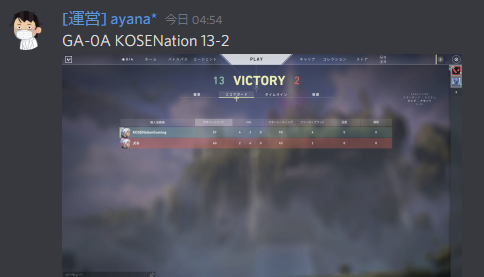
\includegraphics[width=70mm]{result.png}
	                            \hspace{1.6cm} [1]投稿内容の例
	                        \end{center}
	                    \end{minipage}

	                    \begin{minipage}{0.5\hsize}
	                        \begin{center}
                                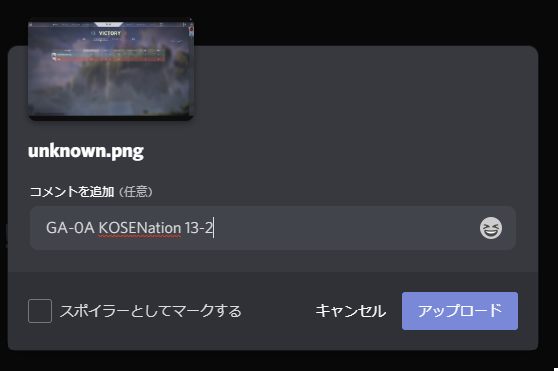
\includegraphics[width=70mm]{example.png}
	                            \hspace{1.6cm} [2]貼り付け方の例
	                        \end{center}
	                    \end{minipage}
	                \end{tabular}
	            \end{center}
            \end{figure}
            敗北したチーム側は勝利報告が勝利したチームによって正しく行われているかを必ず確認してください。
            異議がありましたら運営までご連絡ください。

\end{document}